\documentclass{beamer}

%Packages
\usepackage[utf8]{inputenc}
\usepackage{hyperref}
\usepackage{amssymb}

\newcommand{\realnz}{\mathbb{R}^{\*}}
\usepackage{svg}

%META-INFORMATION
\title{Semantic Search for Quantity Expressions}
\author{Tom Wiesing\\\ \\Supervisor: Michael Kohlhase\\Co-supervisor: Tobias Preusser}
\date{May 20, 2015 \\110392 Guided Research Applied and Computational Mathematics \& Thesis}

\begin{document}
  %TITLEPAGE
  \frame{\titlepage}

  %OVERVIEW
  \begin{frame}{Overview}
    \pause
    \begin{columns}[T]
      \begin{column}[T]{7cm}
        \begin{itemize}[<+->]
          \item Motivation: Problem and State Of The Art
          \item Our Approach: Structure Of The Search Engine
          \begin{itemize}
            \item The Unit System
            \item The Search Algorithm
          \end{itemize}
          \item Conclusion: The Implementation
          \item Time for Questions
        \end{itemize}
      \end{column}
    \end{columns}
  \end{frame}

  %MOTIVATION
  \begin{frame}{Motivation (1)}
    \begin{itemize}[<+->]
      \item We use units every day
      \item We encounter them everywhere:
      \begin{itemize}[<+->]
        \item When driving, there are speed limits, for example: \raisebox{-0.5\height}{
\includegraphics[width=10mm]{imgs/sign60.png}} $\frac{\text{km}}{\text{h}}$ % http://www.gettingaroundgermany.info/g_imgs/z274.gif
        \item When baking, it often says in recepies something like: ``add 3 tea spoons of sugar''
        \item When shopping for shoes there are different sizes
      \end{itemize}
      \item In scientific papers they occur a lot
      \item everything which somehow models a real system has at least one quantity expression
      \item everything is quantified
    \end{itemize}
  \end{frame}

  \begin{frame}{Motivation (2)}
    \begin{itemize}[<+->]
      \item But where is the problem?
      \item Within one paper only a handful of units is used
      \item In general there are \textbf{a lot} of \textbf{different} units to describe \textbf{the same} quantity
      \item Just for lengths: \pause \textit{Meter}, \pause \textit{Inch}, \pause \textit{Foot}, \pause \textit{Mile}, \pause \textit{Nautical Mile}, \pause $\dots$
      \item This can cause problems when not converting properly
      \item Mars Climate Orbiter (1999) \\ 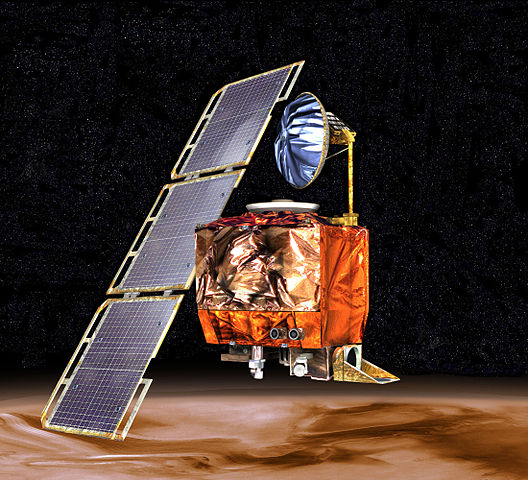
\includegraphics[width=50mm]{imgs/mco.jpg}
      % http://upload.wikimedia.org/wikipedia/commons/thumb/1/19/Mars_Climate_Orbiter_2.jpg/528px-Mars_Climate_Orbiter_2.jpg
      \item Different Units are a big problem
    \end{itemize}
  \end{frame}

  \begin{frame}{Motivation (3)}
    \pause
    \begin{itemize}[<+->]
      \item What is the most common solution?
      \item Unit Converters
      \begin{itemize}[<+->]
        \item There are a lot of these \\ 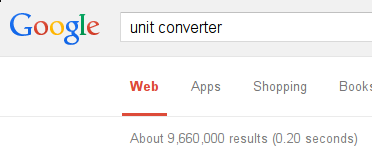
\includegraphics[width=40mm]{imgs/google.png}
        \item Google itself has one integrated \\ 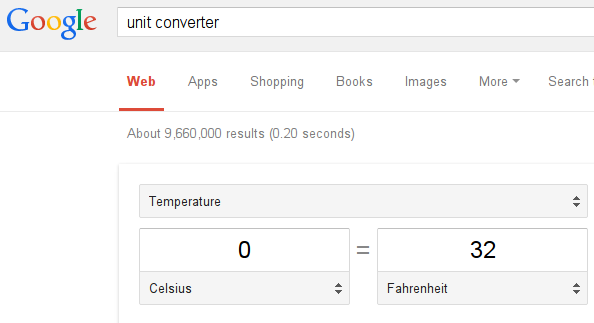
\includegraphics[width=40mm]{imgs/googleuc.png}
      \end{itemize}
    \end{itemize}
  \end{frame}

  \begin{frame}{Motivation (4)}
    \begin{itemize}[<+->]
      \item user needs to find out that conversion is required
      \item both input \textbf{and} output units need to be \textbf{given}
      \item this is not integrated into the search process itself
      \item Wouldn't it be nice:
      \begin{itemize}[<+->]
        \item when searching for $25\ \frac{\text{m}}{\text{s}}$
        \item we also find $90\ \frac{\text{km}}{\text{h}}$
        \item we did not have to search for all the representations of the same quantity expression
      \end{itemize}
      \item This is the kind of search engine we have built
    \end{itemize}
  \end{frame}

  %APPROACH
  \begin{frame}{Our Approach (1)}
    \begin{itemize}[<+->]
      \item What components do we need for a semantic search engine?
      \begin{enumerate}[<+->]
        \item A \textit{Unit System} that is aware of the different representations of a QE
        \item A \textit{Spotter} that finds representations of QEs inside documents
        \item A \textit{Search Algorithm} that given a QE finds all its representations in the system
        \item A \textit{Frontend} that allows queries to be made
      \end{enumerate}

      \item Spotter is done by \textit{Stiv Sherko}
      \item We only need to worry about the \textit{Unit System}, the \textit{Search Algorithm} and the \textit{Frontend}
      \item For the first two points, we use a meta-mathematical approach
    \end{itemize}
  \end{frame}


  \begin{frame}{Our Approach (2)}
    \begin{itemize}[<+->]
      \item We use a meta-mathematical model
      \item This is a model that can be used to describe mathematics
      \item We go over this fairly quickly due to time constraints
      \item Definitions (= Constants) are contained inside \textit{theories}
      \item A \textit{Term} is an expression written using definitions from a Theory
      \item Theories can be related using \textit{Imports} and \textit{Views}
      \item An Import makes Constants from one theory available in another
      \item A View is a truth-preserving mapping from Constants of one theory to another
      \item With the help of these relation we can make a \textit{Theory Graph}
      \item You will see examples with our unit system
      \item \textit{MMT} is a software that allows us to make use of these concepts
      \item It is easy to write down your own theories and related them with views
    \end{itemize}
  \end{frame}
    %Unit System
  \begin{frame}{Our Approach: The Unit System (1)}
    \begin{itemize}[<+->]

      \item Let us start with building a theory of Quantity Expressions
      \item We orient ourselves on the SI specification
      \item Each quantity has a dimension
      \item According to SI there are 7 basic ones:
      \begin{itemize}
        \item length
        \item mass
        \item time
        \item electric current
        \item temperature
        \item luminous intensity
        \item amount of substance
      \end{itemize}
      \item but there are also quantities where we just \textit{count}
      \item and \textit{dimensionless quantities} (such as Information)
      \item so we have 9 basic dimensions
    \end{itemize}
  \end{frame}

  \begin{frame}{Our Approach: The Unit System (2)}
    \begin{itemize}[<+->]
      \item we can also multiply these to get new dimensions
      \item such as area $=$ length $\cdot{}$ length
      \item similarly we can divide dimensions
      \item such as velovity $= \frac{\text{length}}{\text{time}}$
      \item We can use this to get a \textit{Theory of Dimensions}:
    \end{itemize}
  \end{frame}
  \begin{frame}{Our Approach: The Unit System (3)}
    \begin{center}
      \begin{tabular}{|l l l|}
        \hline
        \textsf{Dimension} & &\\\hline
        $\mathsf{dim}$ & $:$ & $ \mathsf{type}$\\

        $\mathsf{none}$ & $:$ & $ \mathsf{dim}$\\
        $\mathsf{count}$ & $:$ & $ \mathsf{dim}$\\
        $\mathsf{length}$ & $:$ & $ \mathsf{dim}$\\
        $\mathsf{mass}$ & $:$ & $ \mathsf{dim}$\\
        $\mathsf{time}$ & $:$ & $ \mathsf{dim}$\\
        $\mathsf{current}$ & $:$ & $ \mathsf{dim}$\\
        $\mathsf{temperature}$ & $:$ & $ \mathsf{dim}$\\
        $\mathsf{luminous}$ & $:$ & $ \mathsf{dim}$\\
        $\mathsf{amount}$ & $:$ & $ \mathsf{dim}$\\

        $\cdot{}$ & $:$ & $ \mathsf{dim} \rightarrow \mathsf{dim} \rightarrow \mathsf{dim}$\\
        $/$ & $:$ & $ \mathsf{dim} \rightarrow \mathsf{dim} \rightarrow \mathsf{dim}$\\\hline
      \end{tabular}
  \end{center}
\end{frame}

  \begin{frame}{Our Approach: The Unit System (4)}
    \begin{itemize}[<+->]
      \item how can we formalise a quantity expressions?
      \item In our model QEs can be one of the following:
      \begin{enumerate}
        \item (1 times) a \textit{primitive unit}, such as Meter
        \item A \textit{multiplication} of a (real) number with an existing QE, such as $5\ \text{Meter}$
        \item A \textit{division} of an existing QE by a (non-zero real) number (equivalent to the above)
        \item The \textit{product} of two existing QEs such as $\text{Newton} \cdot{} \text{Second}$
        \item The \textit{sum} of two existing QEs (of the same dimension)
        \item The \textit{quotient} of two existing QEs such as $1\ \frac{\text{Meter}}{\text{Second}}$
      \end{enumerate}
      \item this results in the following \textit{Theory of Quantity Expressions}:
    \end{itemize}
  \end{frame}

  \begin{frame}{Our Approach: The Unit System (5)}
    \begin{center}
      \begin{tabular}{|l l l|}
        \hline
        \textsf{Quantity Expression} & &\\\hline
        $ \mathsf{import \ Dimension}$ &&\\\hline
        $\mathsf{QE}$ & $:$ & $ \mathsf{dim} \rightarrow \mathsf{type}$\\
        $\mathsf{QENMul}$& $:$ & $ \forall x : \mathsf{dim} . \realnz \rightarrow \mathsf{QE}\left( x\right) \rightarrow \mathsf{QE}\left( x\right)$\\
        $\mathsf{QENDiv}$& $:$ & $ \forall x : \mathsf{dim} . \mathsf{QE}\left( x\right) \rightarrow \realnz \rightarrow \mathsf{QE}\left( x\right)$\\

        $\mathsf{QEAdd}$& $:$ & $ \forall x : \mathsf{dim} . \mathsf{QE}\left( x\right) \rightarrow \mathsf{QE}\left( x\right) \rightarrow \mathsf{QE} \left( x \right)  $\\
        $\mathsf{QEMul}$& $:$ & $ \forall x, y : \mathsf{dim} . \mathsf{QE}\left( x\right) \rightarrow \mathsf{QE}\left( y\right) \rightarrow \mathsf{QE} \left( x \cdot{} y \right)  $\\
        $ \mathsf{QEDiv}$& $:$ & $ \forall x, y : \mathsf{dim} . \mathsf{QE}\left( x\right) \rightarrow \mathsf{QE}\left( y\right) \rightarrow \mathsf{QE} \left( \frac{x}{y} \right)  $\\\hline
      \end{tabular}
    \end{center}
  \end{frame}

  \begin{frame}{Our Approach: The Unit System (6)}
    \begin{itemize}[<+->]
      \item we can now easily create theories that define Units, such as a Meter Theory:
      \item
          \begin{tabular}{|l l l|}
            \hline
            \textsf{Meter} &&\\\hline
            $ \mathsf{import \ Quantity\ Expression}$ &&\\
            \hline
            $\mathsf{Meter}$ & $:$ & $ \mathsf{QE} \left( \mathsf{length} \right)$\\\hline
          \end{tabular}
    \item we can also define some non-metric lengths:
    \item
      \begin{tabular}{|l|}
        \hline
        \textsf{Non SI Lengths}\\\hline
        $ \mathsf{import \ Quantity\ Expression}$\\
        \hline
        $\mathsf{Thou} : \mathsf{QE}\left( \mathsf{length} \right)$\\
        $\mathsf{Foot} = \mathsf{QENMul} \left( 1000, \mathsf{Thou} \right)$\\
        $\mathsf{Yard} = \mathsf{QENMul} \left( 3, \mathsf{Foot} \right)$\\
        $\mathsf{Chain} = \mathsf{QENMul} \left( 22, \mathsf{Yard} \right)$\\
        $\mathsf{Furlong} = \mathsf{QENMul} \left( 10, \mathsf{Chain} \right)$\\
        $\mathsf{Mile} = \mathsf{QENMul} \left( 8, \mathsf{Furlong} \right)$\\
        \hline
      \end{tabular}
    \end{itemize}
  \end{frame}

  \begin{frame}{Our Approach: The Unit System (7)}
    \begin{itemize}[<+->]
      \item We also need to be able to compare units
      \item We use \textit{Views} (mappings between theories) for this
      \item In this case we use the view
        \[
          \psi = \left\{\begin{array}{l}
            \mathsf{Thou} \mapsto \mathsf{QENMul} \left( 0.0000254, \mathsf{Meter} \right)
          \end{array}\right\}
        \]
      \item This allows us to convert quantity expression representations between different units
      \item We have a big (easily extensible) theory graph of unit theories
      \item Here is a small part of it
    \end{itemize}
  \end{frame}

  \begin{frame}{Our Approach: The Unit System (6)}
    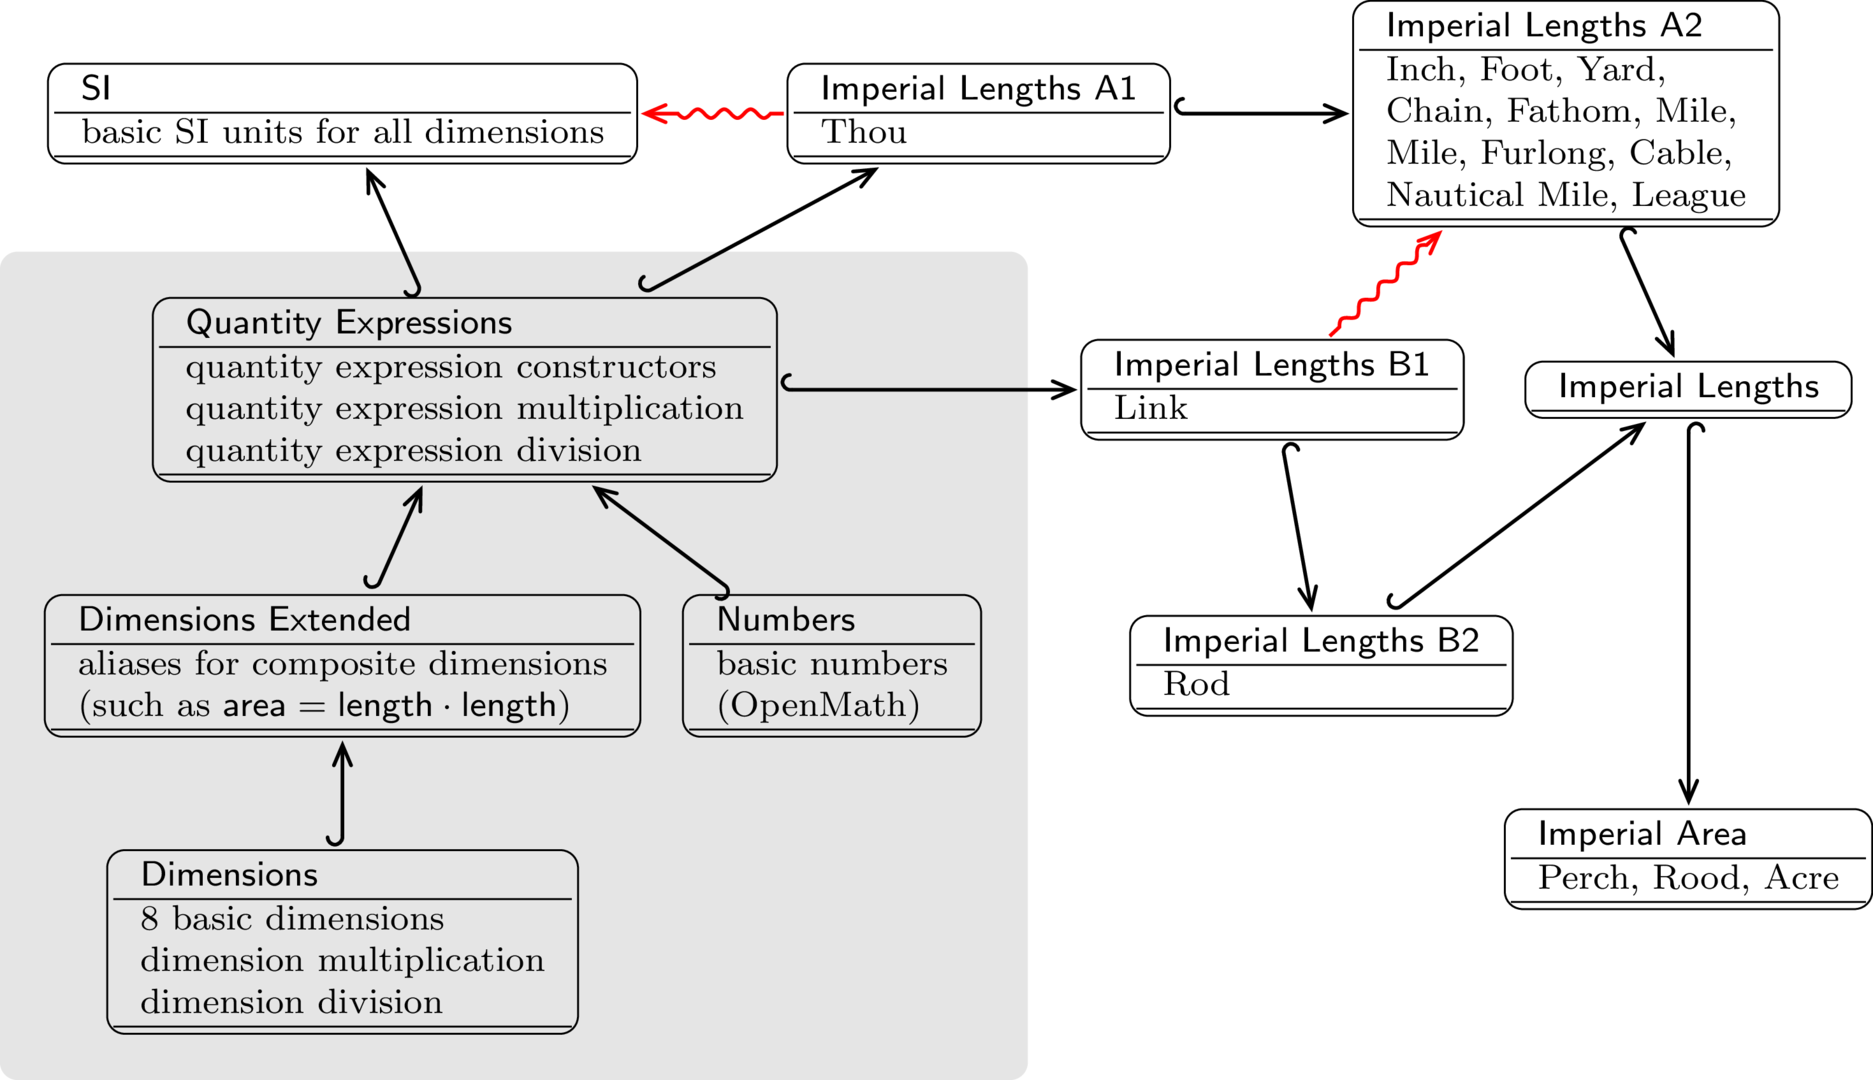
\includegraphics[width=90mm]{imgs/graph1.png}
  \end{frame}

  % The Search Algorithm
  \begin{frame}{Our Approach: The Search Algorithm (1)}
    \begin{itemize}[<+->]
      \item Let us build a search algorithm
      \item We are given a \textit{query} and want to find all equivalent quantity expressions
      \item We already have a list of quantity expressions from the spotter
      \item We just need an efficient way to check if two QEs are the same
      \item We can just bring QEs to a normal form
      \item and then have an efficient index
    \end{itemize}
  \end{frame}

  \begin{frame}{Our Approach: The Search Algorithm (2)}
    \begin{itemize}[<+->]
      \item A normal form should consist of two components:
      \item A \textit{scalar} component and a (scalar-free) \textit{unit} component
      \item The \textit{unit} component should be in standard units (in our case SI)
      \item For this we use 2-step-normalisation
    \end{itemize}
  \end{frame}

  \begin{frame}{Our Approach: The Search Algorithm (3)}
    \begin{itemize}[<+->]
      \item Example: Normalise $42 \frac{\text{Furlong}}{\text{Fortnight}}$
      \item First, turn all units into standard units by finding an appropriate path in the \textit{theory graph} of units
      \item $\text{Furlong} \pause = 10\ \text{Chain} \pause = 10 \left( 22\ \text{Yard}\right) \pause = \dots = 10 \left( 22 \left( 3 \left( 12 \left( 1000 \left( 0.0000254\ \text{Meter} \right) \right) \right) \right)\right) $
      \item $\text{Fortnight} = \left( 2 \left( 7 \left( 24 \left( 60 \left( 60\ \text{Second} \right) \right) \right) \right) \right) $
      \item Substitute this back into the original expression
      \item $42 \frac{10 \left( 22 \left( 3 \left( 1000 \left( 0.0000254\ \text{Meter} \right) \right) \right)\right)}{ 2 \left( 7 \left( 24 \left( 60 \left( 60\ \text{Second} \right) \right) \right) \right)}$
      \item Then extract the \textit{scalar} component and compute it:
      \item $ 42 \frac{10 \left( 22 \left( 3 \left( 12 \left( 1000 \left( 0.0000254 \right) \right) \right) \right)\right)}{ 2 \left( 7 \left( 24 \left( 60 \left( 60\right) \right) \right) \right)} = 0.006985 $
      \item Continue by extracting the \textit{unit} component: $\frac{\text{Meter}}{\text{Second}}$
      \item Finally multiply these components to get the standard form:
      \item $0.006985\ \frac{\text{Meter}}{\text{Second}}$
    \end{itemize}
  \end{frame}

  \begin{frame}{Our Approach: The Search Algorithm (4)}
    \begin{itemize}[<+->]
      \item We can then compare the spotted QEs with the query via directly comparing normal forms
      \item To save time, we \textit{cache} the normal form of each unit
      \item We can also \textit{cache} the normal forms of the QEs found by the spotter
      \item Important: We choose SI units for the standard form
      \item This is not required. We could also choose to use imperial units as a normal form
      \item Our unit graph is flexible enough so that we can actually do that
    \end{itemize}
  \end{frame}

  \begin{frame}{Our Approach: The Search Algorithm (5)}
    \begin{itemize}[<+->]
      \item We can then compare the spotted QEs with the query via directly comparing normal forms
      \item To save time, we \textit{cache} the normal form of each unit
      \item We can also \textit{cache} the normal forms of the QEs found by the spotter
      \item Important: We choose SI units for the standard form
      \item This is not required. We could also choose to use imperial units as a normal form
      \item Our unit graph is flexible enough so that we can actually do that
    \end{itemize}
  \end{frame}

  \begin{frame}{Conclusion: The Implementation}
    \begin{itemize}[<+->]
      \item We have the following implemented components:
      \item The frontend, written in HTML, CSS, JavaScript
      \item when queried, this sends a QE to the backend
      \item The backend, written in scala, uses MMT to normalise this expression
      \item and then searches the harvests (provided by Stiv's Spotter)
      \item Finally the frontend displays a list of results
    \end{itemize}
  \end{frame}

  \begin{frame}{Conclusion: The Implementation (2)}
    \begin{itemize}[<+->]
      \item The unit Graph are extensible
      \item The user does not need to think about what units are inside the documents
      \item Time for a demo (if there is still time)
    \end{itemize}
  \end{frame}

  \begin{frame}{Time for Questions}
    \huge{Thank You For Listening!}
    \\\ \\\ \\\
    \tiny{
    Image sources: \\
      \begin{itemize}
        \item \url{http://www.gettingaroundgermany.info/g_imgs/z274.gif}
        \item \url{http://upload.wikimedia.org/wikipedia/commons/thumb/1/19/Mars_Climate_Orbiter_2.jpg/528px-Mars_Climate_Orbiter_2.jpg}
      \end{itemize}
    }

  \end{frame}

  %Need pdf2svg && comvert to run Makefile
\end{document}
